\subsection{Trusses}

\begin{figure}
  \begin{center}
  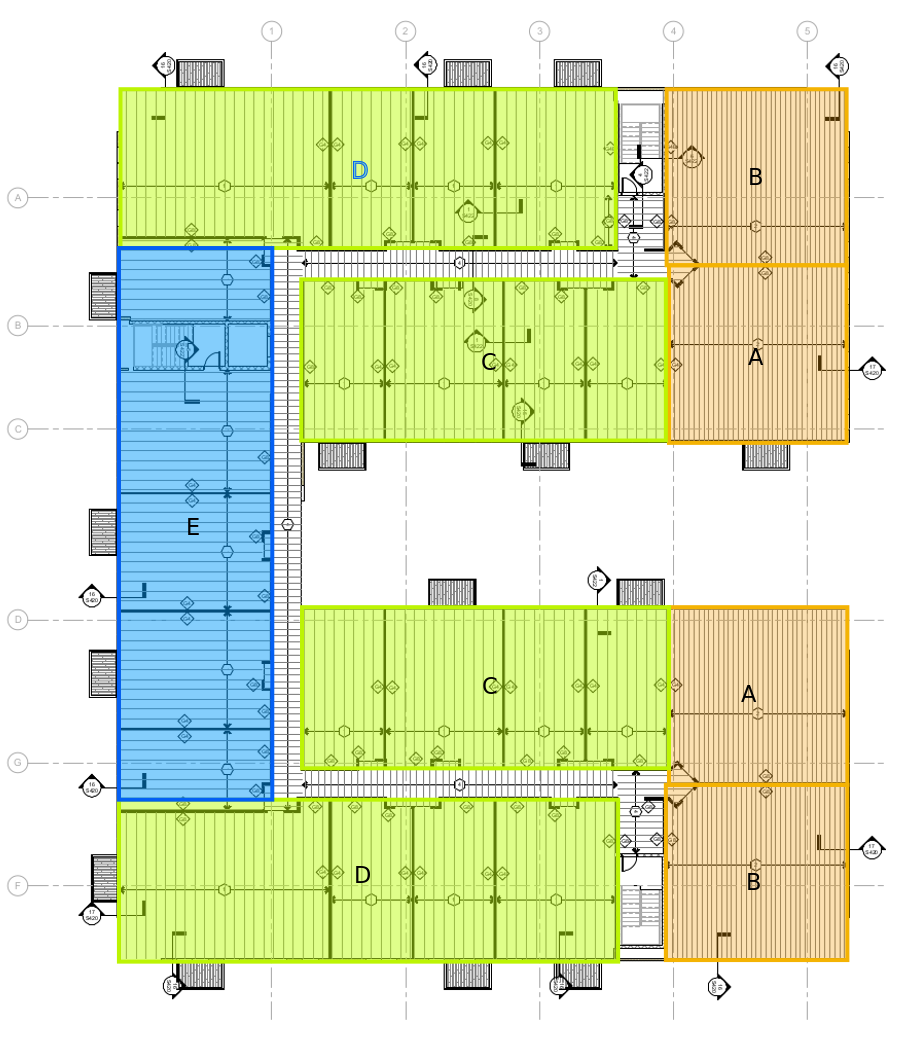
\includegraphics[width=120mm]{figures/3rd_floor_truss_key_plan}
  \end{center}
  \caption{Trusses key plan.}\label{fg_3rd_floor_truss_key_plan}
\end{figure}

\subsubsection{Trusses A and B. Roof}
The deflection results for those trusses (see figure \ref{fg_roof_truss_AB}) are as follows:

\begin{center}
  \begin{scriptsize}
  \begin{tabular}{|l|c|c|c|c|c|c|}
    \hline
    \textbf{Load} & \textbf{truss} & \multicolumn{2}{c|}{\textbf{deflection}} & \textbf{truss} & \multicolumn{2}{c|}{\textbf{deflection}} \\
    \hline
EQ1608 & roof(A): & -1.94 mm & (L/5782; L= 11.22 m) & roof(B): &-1.12 mm & (L/9586; L= 10.77 m) \\
EQ1609 & roof(A): & -5.63 mm & (L/1994; L= 11.22 m) & roof(B): & -3.82 mm & (L/2819; L= 10.77 m) \\
EQ1610 & roof(A): & -9.66 mm & (L/1161; L= 11.22 m) & roof(B): & -6.76 mm & (L/1591; L= 10.77 m) \\
EQ1611 & roof(A): & -10.49 mm & (L/1069; L= 11.22 m) & roof(B): & -7.38 mm & (L/1459; L= 10.77 m) \\
EQ1612 & roof(A): & 0.99 mm & (L/11391; L= 11.22 m) & roof(B): & 1.02 mm & (L/10598; L= 10.77 m) \\
EQ1613 & roof(A): & -8.30 mm & (L/1352; L= 11.22 m) & roof(B): & -5.77 mm & (L/1865; L= 10.77 m) \\
EQ1615 & roof(A): & 1.76 mm & (L/6370; L= 11.22 m) & roof(B): & 1.47 mm & (L/7348; L= 10.77 m) \\
LIVE & roof(A): & -3.69 mm & (L/3044; L= 11.22 m) & roof(B): & -2.69 mm & (L/3995; L= 10.77 m) \\
\hline
  \end{tabular}
  \end{scriptsize}
\end{center}

\noindent The truss depth is allways greater than 24 inches due to the geometry of the roof. The spacing of the trusses is 12 inches.

\begin{figure}
  \begin{center}
  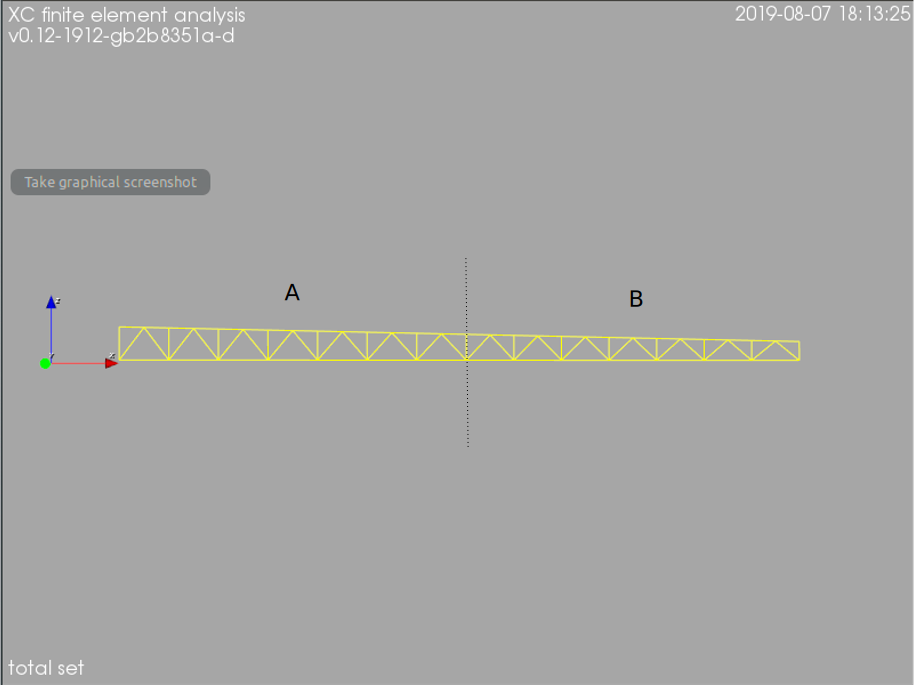
\includegraphics[width=120mm]{figures/roof_truss_AB}
  \end{center}
  \caption{Roof trusses at zones A and B (see key plan in figure \ref{fg_3rd_floor_truss_key_plan}).}\label{fg_roof_truss_AB}
\end{figure}

\subsubsection{Trusses A and B. Floors}
The deflection results for those trusses (see figure \ref{fg_floor_truss_AB}) are as follows:

\begin{center}
  \begin{scriptsize}
  \begin{tabular}{|l|c|c|c|c|c|c|}
    \hline
    \textbf{Load} & \textbf{truss} & \multicolumn{2}{c|}{\textbf{deflection}} & \textbf{truss} & \multicolumn{2}{c|}{\textbf{deflection}} \\
    \hline
EQ1608 & A & -9.14 mm & (L/1228; L= 11.22 m)  & B & -7.75 mm & (L/1389; L= 10.77 m) \\
EQ1609 & A & -26.45 mm & (L/424; L= 11.22 m) & B & -22.46 mm & (L/479; L= 10.77 m) \\
EQ1610 & A & -9.13 mm & (L/1228; L= 11.22 m) & B & -7.74 mm & (L/1389; L= 10.77 m) \\
EQ1611 & A & -22.12 mm & (L/507; L= 11.22 m) & B & -18.78 mm & (L/573; L= 10.77 m) \\
EQ1612 & A & -9.14 mm & (L/1228; L= 11.22 m) & B & -7.75 mm & (L/1389; L= 10.77 m) \\
EQ1613 & A & -22.12 mm & (L/507; L= 11.22 m) & B & -18.78 mm & (L/573; L= 10.77 m) \\
EQ1615 & A & -5.48 mm & (L/2047; L= 11.22 m) & B & -4.65 mm & (L/2315; L= 10.77 m) \\
LIVE & A & -17.32 mm & (L/648; L= 11.22 m) & B & -14.71 mm & (L/731; L= 10.77 m) \\
\hline
  \end{tabular}
  \end{scriptsize}
\end{center}
\noindent The truss depth is 24 inches and the spacing of the trusses is 12 inches.
\begin{figure}
  \begin{center}
  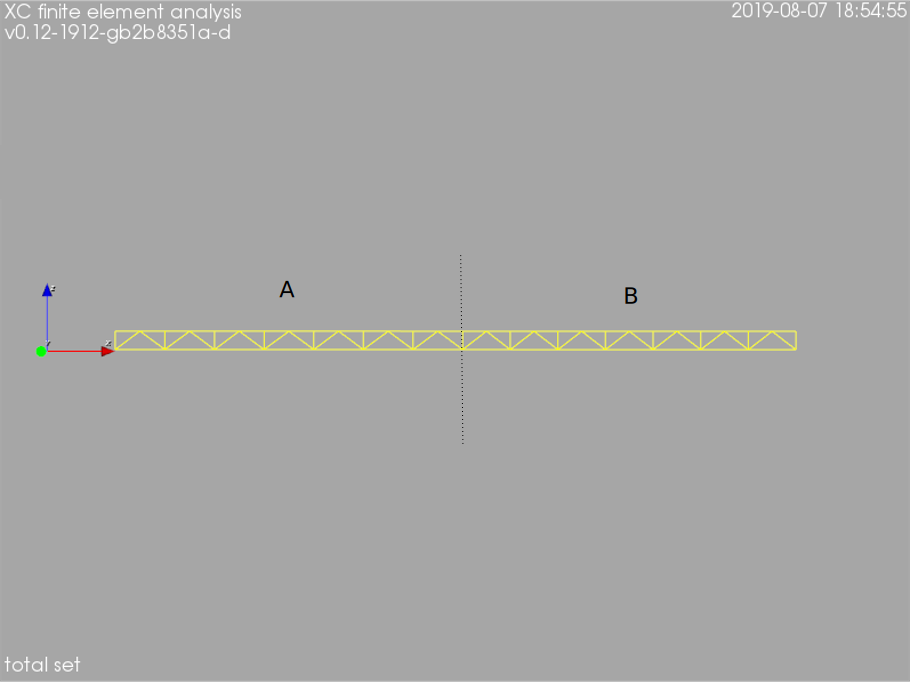
\includegraphics[width=120mm]{figures/floor_truss_AB}
  \end{center}
  \caption{Floor trusses at zones A and B (see key plan in figure \ref{fg_3rd_floor_truss_key_plan}).}\label{fg_floor_truss_AB}
\end{figure}

\subsubsection{Trusses C and D. Roof}
The deflection results for those trusses (see figure \ref{fg_roof_truss_CD}) are as follows:

\begin{center}
  \begin{scriptsize}
  \begin{tabular}{|l|c|c|c|c|c|c|}
    \hline
    \textbf{Load} & \textbf{truss} & \multicolumn{2}{c|}{\textbf{deflection}} & \textbf{truss} & \multicolumn{2}{c|}{\textbf{deflection}} \\
    \hline
EQ1608 & roof(C) & -2.92 mm & (L/3420; L= 10.00 m) & roof(D) & -5.24 mm & (L/1822; L= 9.55 m) \\
EQ1609 & roof(C) & -7.42 mm & (L/1347; L= 10.00 m) & roof(D) & -11.87 mm & (L/803; L= 9.55 m) \\
EQ1610 & roof(C) & -12.34 mm & (L/810; L= 10.00 m) & roof(D) & -19.13 mm & (L/498; L= 9.55 m) \\
EQ1611 & roof(C) & -13.36 mm & (L/748; L= 10.00 m) & roof(D) & -20.64 mm & (L/462; L= 9.55 m) \\
EQ1612 & roof(C) & 0.64 mm & (L/15512; L= 10.00 m) & roof(D) & 0.03 mm & (L/323264; L= 9.55 m) \\
EQ1613 & roof(C) & -10.68 mm & (L/936; L= 10.00 m) & roof(D) & -16.69 mm & (L/572; L= 9.55 m) \\
EQ1615 & roof(C) & 1.81 mm & (L/5512; L= 10.00 m) & roof(D) & 2.12 mm & (L/4493; L= 9.55 m) \\
LIVE & roof(C) & -4.50 mm & (L/2224; L= 10.00 m) & roof(D) & -6.64 mm & (L/1438; L= 9.55 m) \\
\hline
  \end{tabular}
  \end{scriptsize}
\end{center}

\noindent The truss depth is allways greater than 24 inches due to the geometry of the roof. The spacing of the trusses is 24 inches. The spacing of the joists is 32 inches. 

\begin{figure}
  \begin{center}
  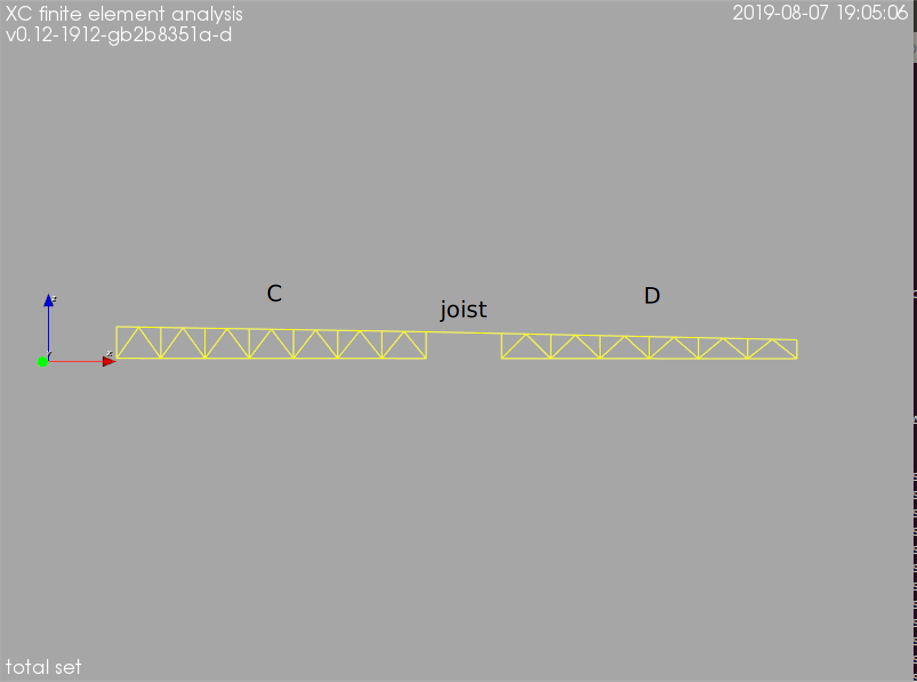
\includegraphics[width=120mm]{figures/roof_truss_CD}
  \end{center}
  \caption{Roof trusses at zones C and D (see key plan in figure \ref{fg_3rd_floor_truss_key_plan}).}\label{fg_roof_truss_CD}
\end{figure}

\subsubsection{Trusses C and D. Floors}
The deflection results for those trusses (see figure \ref{fg_floor_truss_CD}) are as follows:

\begin{center}
  \begin{scriptsize}
  \begin{tabular}{|l|c|c|c|c|c|c|}
    \hline
    \textbf{Load} & \textbf{truss} & \multicolumn{2}{c|}{\textbf{deflection}} & \textbf{truss} & \multicolumn{2}{c|}{\textbf{deflection}} \\
    \hline
EQ1608 & C & -10.00 mm & (L/982; L= 9.82 m) & D & -8.93 mm & (L/1048; L= 9.37 m) \\
EQ1609 & C & -26.93 mm & (L/364; L= 9.82 m) & D & -24.04 mm & (L/389; L= 9.37 m) \\
EQ1610 & C & -10.00 mm & (L/982; L= 9.82 m) & D & -8.93 mm & (L/1048; L= 9.37 m) \\
EQ1611 & C & -22.70 mm & (L/432; L= 9.82 m) & D & -20.26 mm & (L/462; L= 9.37 m) \\
EQ1612 & C & -10.00 mm & (L/982; L= 9.82 m) & D & -8.93 mm & (L/1048; L= 9.37 m) \\
EQ1613 & C & -22.70 mm & (L/432; L= 9.82 m) & D & -20.26 mm & (L/462; L= 9.37 m) \\
EQ1615 & C & -6.00 mm & (L/1636; L= 9.82 m) & D & -5.36 mm & (L/1747; L= 9.37 m) \\
LIVE & C & -16.93 mm & (L/580; L= 9.82 m) & D & -15.11 mm & (L/620; L= 9.37 m) \\
\hline
  \end{tabular}
  \end{scriptsize}
\end{center}

\begin{figure}
  \begin{center}
  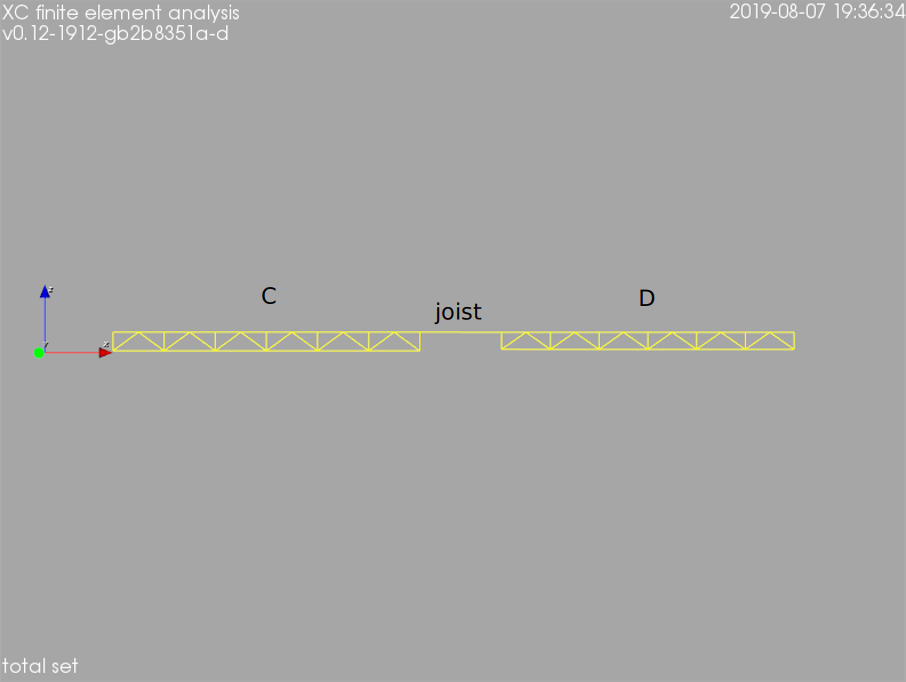
\includegraphics[width=120mm]{figures/floor_truss_CD}
  \end{center}
  \caption{Floor trusses at zones C and D (see key plan in figure \ref{fg_3rd_floor_truss_key_plan}).}\label{fg_floor_truss_CD}
\end{figure}

\noindent The truss depths are 24 inches for the C truss 22 inches for the D truss. The spacing of the trusses is 12 inches. The spacing of the joists is 32 inches. 

\subsubsection{Truss E. Roof}
The deflection results for those trusses (see figure \ref{fg_roof_truss_E}) are as follows:

\begin{center}
  \begin{scriptsize}
  \begin{tabular}{|l|c|c|c|c|c|c|}
    \hline
    \textbf{Load} & \textbf{truss} & \multicolumn{2}{c|}{\textbf{deflection}} \\
    \hline
EQ1608 & 3E & -4.67 mm & (L/2025; L= 9.47 m) \\
EQ1609 & 3E & -11.56 mm & (L/819; L= 9.47 m) \\
EQ1610 & 3E & -19.09 mm & (L/496; L= 9.47 m) \\
EQ1611 & 3E & -20.65 mm & (L/458; L= 9.47 m) \\
EQ1612 & 3E & 0.79 mm & (L/11978; L= 9.47 m) \\
EQ1613 & 3E & -16.55 mm & (L/572; L= 9.47 m) \\
EQ1615 & 3E & 2.66 mm & (L/3559; L= 9.47 m) \\
LIVE & 3E & -6.89 mm & (L/1375; L= 9.47 m) \\
\hline
  \end{tabular}
  \end{scriptsize}
\end{center}

\noindent The truss depth is allways greater than 24 inches due to the geometry of the roof. The spacing of the trusses is 24 inches. The spacing of the joists is 32 inches.

\begin{figure}
  \begin{center}
  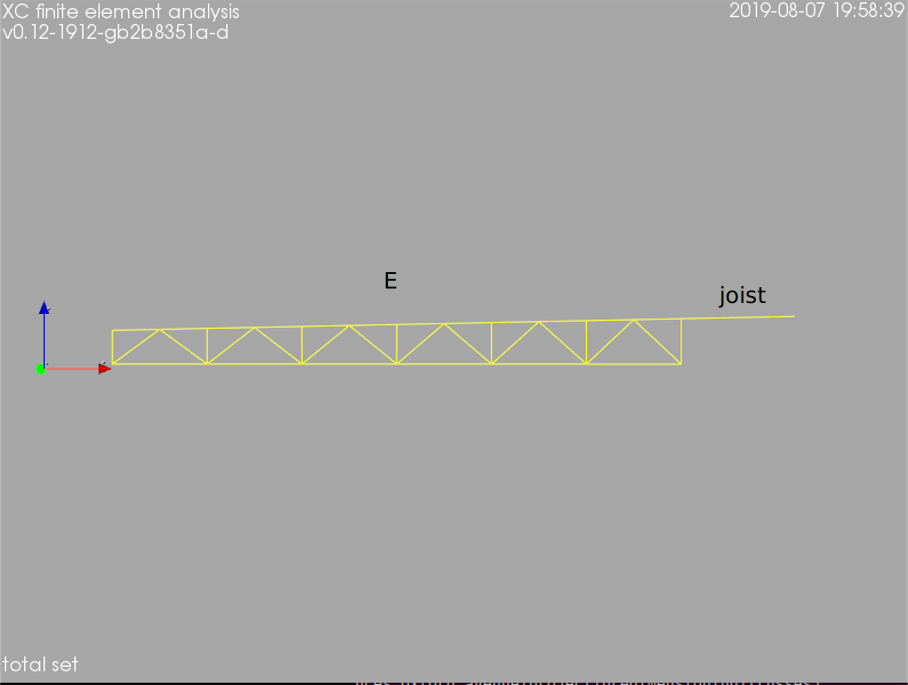
\includegraphics[width=120mm]{figures/roof_truss_E}
  \end{center}
  \caption{Roof truss at zone E (see key plan in figure \ref{fg_3rd_floor_truss_key_plan}).}\label{fg_roof_truss_E}
\end{figure}

\subsubsection{Truss E. Floor}
The deflection results for those trusses (see figure \ref{fg_floor_truss_E}) are as follows:

\begin{center}
  \begin{scriptsize}
  \begin{tabular}{|l|c|c|c|c|c|c|}
    \hline
    \textbf{Load} & \textbf{truss} & \multicolumn{2}{c|}{\textbf{deflection}} \\
    \hline
EQ1608 & 2E & -8.65 mm & (L/1095; L= 9.47 m) \\
EQ1609 & 2E & -23.30 mm & (L/406; L= 9.47 m) \\
EQ1610 & 2E & -8.65 mm & (L/1095; L= 9.47 m) \\
EQ1611 & 2E & -19.63 mm & (L/482; L= 9.47 m) \\
EQ1612 & 2E & -8.65 mm & (L/1095; L= 9.47 m) \\
EQ1613 & 2E & -19.63 mm & (L/482; L= 9.47 m) \\
EQ1615 & 2E & -5.19 mm & (L/1825; L= 9.47 m) \\
LIVE & 2E & -14.65 mm & (L/646; L= 9.47 m) \\
\hline
  \end{tabular}
  \end{scriptsize}
\end{center}

\noindent The truss depth 24 inches. The spacing of the trusses is 24 inches and the spacing of the joists is 32 inches.

\begin{figure}
  \begin{center}
  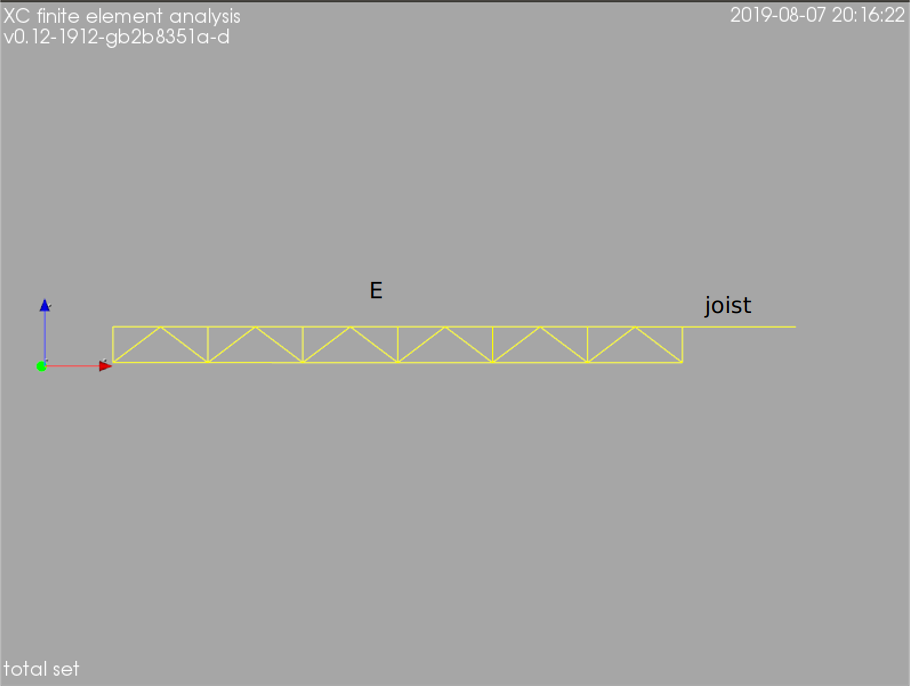
\includegraphics[width=120mm]{figures/floor_truss_E}
  \end{center}
  \caption{Floor truss at zone E (see key plan in figure \ref{fg_3rd_floor_truss_key_plan}).}\label{fg_floor_truss_E}
\end{figure}
